% ============================================================
\clearpage
\section*{Appendix B. Worked Examples}
\addcontentsline{toc}{section}{Appendix B. Worked Examples}
% ============================================================

This appendix provides concrete examples illustrating the categorical
interpretations developed in the paper. The goal is to anchor the abstract
definitions (functors, fibrations, oplax structure) in realistic CEP
workflows.

% ------------------------------------------------------------
\subsection*{B.1 Normalization and Canonicalization Example}
% ------------------------------------------------------------

Consider an entity with the following unnormalized fields:

\begin{mdframed}
    \textbf{Name:} ``City of Springfield'' \\
    \textbf{Address:} ``123 Lincoln Ave'' \\
    \textbf{Country:} ``US'' \\
    \textbf{Date:} (none)
\end{mdframed}

After running the normalization functor
\[
    \mathcal{F}_{normalize} : \mathbf{R}_{raw} \to \mathbf{R}_{canon},
\]
we obtain:

\begin{mdframed}
    \textbf{Name:} ``city of springfield'' (lowercased) \\
    \textbf{Address:} ``123 lincoln ave'' \\
    \textbf{Country:} ``US'' \\
    \textbf{Date:} ``1900-01-01'' (jurisdiction-default)
\end{mdframed}

The canonicalization functor
\[
    \mathcal{C} : \mathbf{R}_{canon} \to \mathbf{C}
\]
then produces the canonical string:
\[
    \mathcal{C}(R) =
    \texttt{city of springfield|123 lincoln ave|US|1900-01-01}.
\]

Applying the hashing endofunctor $H$ yields:
\[
    \text{SNFEI}(R) = H(\mathcal{C}(R)).
\]

This example demonstrates the strict monoidal behavior of $\mathcal{C}$:
each component is concatenated in a fixed order, independent of
non-identity updates such as revision increments.

% ------------------------------------------------------------
\subsection*{B.2 Envelope Functor and Attestation Naturality}
% ------------------------------------------------------------

Let $P$ be the payload from Example B.1.

\[
    \mathcal{E}(P)
    = \text{Envelope with schema version, timestamps, and revision 1},
\]
\[
    \mathcal{E}'(P)
    = \text{Envelope with cryptographic attestation}.
\]

The natural transformation $\alpha : \mathcal{E} \Rightarrow \mathcal{E}'$
assigns to $P$ a morphism
\[
    \alpha_P : \mathcal{E}(P) \to \mathcal{E}'(P)
\]
representing the application of an attestation (e.g., a digital signature).

If the payload evolves by a valid morphism $f : P \to P'$, the square

\[
    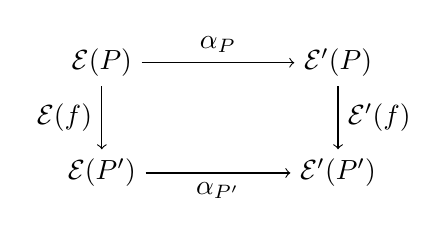
\begin{tikzpicture}[baseline=(current bounding box.center)]
        \node (EP) at (0,0) {$\mathcal{E}(P)$};
        \node (EPP) at (3,0) {$\mathcal{E}'(P)$};
        \node (EPp) at (0,-1.4) {$\mathcal{E}(P')$};
        \node (EPPp) at (3,-1.4) {$\mathcal{E}'(P')$};
        \draw[->] (EP) -- node[above] {$\alpha_P$} (EPP);
        \draw[->] (EPp) -- node[below] {$\alpha_{P'}$} (EPPp);
        \draw[->] (EP) -- node[left] {$\mathcal{E}(f)$} (EPp);
        \draw[->] (EPP) -- node[right] {$\mathcal{E}'(f)$} (EPPp);
    \end{tikzpicture}
\]
commutes, meaning provenance is consistent.

% ------------------------------------------------------------
\subsection*{B.3 Jurisdictional Adapters as Oplax Functors}
% ------------------------------------------------------------

Consider a local schema $\mathbf{J_{local}}$:

\begin{mdframed}
    \textbf{name}, \textbf{state}, \textbf{address}, \textbf{source-system}
\end{mdframed}

and a global CEP vocabulary $\mathbf{J_{global}}$:

\begin{mdframed}
    \textbf{legalName}, \textbf{jurisdictionIso}, \textbf{location.address},
    \textbf{entityTypeUri}, \textbf{status}
\end{mdframed}

An adapter $\mathcal{A}$ maps:

\[
    \mathcal{A}(\texttt{name}) = \texttt{legalName},
    \qquad
    \mathcal{A}(\texttt{state}) = \texttt{jurisdictionIso},
\]
\[
    \mathcal{A}(\texttt{address}) = \texttt{location.address},
\]
while \texttt{source-system} may be mapped into an optional metadata field.

Because optional fields may be dropped or weakened, the functor is oplax:
\[
    \mathcal{A}(x) \otimes \mathcal{A}(y)
    \to \mathcal{A}(x \otimes y)
\]
need not be an isomorphism.

% ------------------------------------------------------------
\subsection*{B.4 Context Tags and Fiber Reindexing}
% ------------------------------------------------------------

Let $R$ be an entity record with SNFEI $s$.

The fiber $\mathbf{CT}_R$ contains allowable tags, e.g.:

\begin{mdframed}
    \texttt{analysis.cluster.membership: "cluster-17"} \\
    \texttt{quality.issue.incomplete\_address: true}
\end{mdframed}

If the base record evolves
\[
    f : R \to R',
\]
then the fibration guarantees a reindexing
\[
    f^\ast : \mathbf{CT}_R \to \mathbf{CT}_{R'}
\]
that keeps tags aligned with the record's identity but never alters $s$.
